\documentclass{beamer}
% Layout, characters, page margins, pictures handling.
\usepackage{graphicx, float}                        % Images
\usepackage{colonequals}                            % poor man's \colonequals
% Math tools
\usepackage{amsmath, amsthm, amsfonts, amssymb}     % A lot of symbols

% References and hyperlinks both in the document and to the web. Needs two compilations in a row.
\usepackage{hyperref, bookmark}

% Commutative diagrams
\usepackage{tikz, tikz-cd}
\usetikzlibrary{calc} % This allows for slightly moving nodes in a tikzpicture, by using ($(m-1-1.east)+(offsetX,offsetY)$) for example.
\usetikzlibrary{arrows, matrix} % I guess

\usepackage{listings}
% \usepackage{fullpage}

% % typesetting
% \usepackage[T1]{fontenc}
% \usepackage{libertine}
% \usepackage[libertine]{newtxmath}
% \usepackage[scaled=0.83]{beramono}
% \usepackage{parskip}                                % To handle paragraph spacing, indentation etc.
% %\usepackage[charter]{mathdesign}
% \usepackage[scaled]{beramono,berasans}
% \usepackage{eucal}
% \usepackage{microtype}
% \frenchspacing

%%%%%%%%%%%%%%%%%%%%%%%%%%%%%%%%%%%%%%%%%%%%%%%%%%%%%%%%%%%%%%%%%%%%%%%%%%%%%%%%%%%%%%%%%%%%%%%%%%%
% Bibliography management. Compile with biber.
\usepackage[backend=biber, datamodel=mrnumber, sortcites]{biblatex}
\addbibresource{bibliography.bib}
\renewcommand*{\bibfont}{\tiny}

\usepackage{gitinfo2}

\newcommand\gitfootnote[1]{% yoinked from Pieter's repo
  \begin{NoHyper}
  \renewcommand\thefootnote{}\footnote{#1}%
  \addtocounter{footnote}{-1}%
  \end{NoHyper}
}

%%%%%%%%%%%%%%%%%%%%%%%%%%%%%%%%%%%%%%%%%%%%%%%%%%%%%%%%%%%%%%%%%%%%%%%%%%%%%%%%%%%%%%%%%%%%%%%%%%%
% Theorems are numbered within sections using a common counter. Do away with ambiguous numbering schemes and assign A number to A thing.
\theoremstyle{plain}
% % \newtheorem{theorem}{Theorem}[section]
% \newtheorem{proposition}[theorem]{Proposition}
% \newtheorem{lemma}[theorem]{Lemma}
% \newtheorem{corollary}[theorem]{Corollary}
% \newtheorem{claim}[theorem]{Claim}
\newtheorem{conjecture}{Conjecture}

% \theoremstyle{remark}
% \newtheorem{remark}[theorem]{Remark}

% \theoremstyle{definition}
% \newtheorem{definition}[theorem]{Definition}
% \newtheorem{example}[theorem]{Example}



%%%%%%%%%%%%%%%%%%%%%%%%%%%%%%%%%%%%%%%%%%%%%%%%%%%%%%%%%%%%%%%%%%%%%%%%%%%%%%%%%%%%%%%%%%%%%%%%%%%%


\newcommand{\iif}{\ensuremath{\Leftrightarrow}}              % If and only if

\renewcommand*{\to}[1][]{\overset{#1}{\rightarrow}} % Arrow with optional label. Use as A \to[label] B


\newcommand{\stable}{-\mathrm{st}}
\newcommand{\semistable}{-\mathrm{sst}}


\newcommand{\dirlim}[1]{                        % Direct limit
    \varinjlim_{\substack{#1}}
    }

\newcommand{\invlim}[1]{                        % Inverse limit
    \varprojlim_{\substack{#1}}
    }

\DeclareMathOperator{\Hom}{Hom}
\DeclareMathOperator{\Ext}{Ext}
\DeclareMathOperator{\dom}{dom}
\DeclareMathOperator{\im}{Im}
\DeclareMathOperator{\GL}{GL}
\DeclareMathOperator{\Mat}{Mat}

% Numbers
\newcommand{\NN}{\mathbb{N}}
\newcommand{\ZZ}{\mathbb{Z}}
\newcommand{\QQ}{\mathbb{Q}}
\newcommand{\RR}{\mathbb{R}}
\newcommand{\CC}{\mathbb{C}}

% Spaces
\renewcommand{\AA}{\mathbb{A}}
\newcommand{\PP}{\mathbb{P}}


% Sheaves

\DeclareMathOperator{\sheafHom}{\mathscr{H}\kern -2.5pt\mathit{om}}
\DeclareMathOperator{\sheafExt}{\mathscr{E}\mathit{xt}}

% various
\newcommand{\tuple}[1]{\mathbf{#1}}
\newcommand{\gianni}[1]{{\color{blue}#1}}

% macros
\DeclareMathOperator{\parameterspace}{R}
\DeclareMathOperator{\modulispace}{M}
\DeclareMathOperator{\group}{\GL_{\tuple{d}}}

\DeclareMathOperator{\HH}{H}

\title{Decomposing quiver moduli - a QuiverTools showcase}
\author{Gianni Petrella - University of Luxembourg}
\institute{MEGA 2024 - MPI MIS Leipzig}
\date{July 29th, 2024}


\begin{document}
\begin{frame}
    \titlepage
% \footnotetex{commit: \texttt{\gitAbbrevHash}\hfil date: \texttt{\gitAuthorIsoDate}\hfil \texttt{\gitReferences}}
\end{frame}

\begin{frame}
    \frametitle{Preamble}
\textbf{Plan}
\begin{enumerate}
    \item What are quiver moduli?
    \item What is \emph{QuiverTools}?
    \item $D^b(Q)$ vs $D^b(M)$
    \item Semiorthogonal embeddings
\end{enumerate} \pause
\vfill
\textbf{Aknowledgements}

This work is supported by the Luxembourg National Research Fund (AFR-17953441)

\end{frame}

\begin{frame}
    \frametitle{Quiver representations}
\begin{definition}
    We work over $k = \bar{k}$, $char(k) = 0$. \pause

    A \emph{quiver}~$Q$ is a finite directed graph, with
    vertices~$Q_0$ and arrows~$Q_1$.

    A \emph{representation}~$V$ of~$Q$ is
    a choice of a $k$-vector space~$V_i$ per vertex~$i$
    and of a linear map~$V_{\alpha}$ per arrow~$\alpha$.
\end{definition} \pause

Once a \emph{dimension vector} $\tuple{d}$ is fixed, a representation
is identified with a point in the \emph{parameter space}
\[
    \parameterspace(Q, \tuple{d})
    \colonequals \bigoplus_{i \to j \in Q_1}
    \Mat_{d_j \times d_i}(k).
\] \pause

The group~${\GL}_{\tuple{d}} \colonequals \bigoplus_{i \in Q_0} \GL_{d_i}$
acts on~$\parameterspace$ by base change. \pause

Orbits are precisely isomorphism classes of representations.
% and two points $V, W$ belong to the
% same orbit precisely when the corresponding representations are isomorphic. \pause
\end{frame}

\begin{frame}
    \frametitle{Quiver moduli via GIT}
A \emph{stability parameter} is~$\theta \in \ZZ^{Q_0}$
for which~$\theta \cdot \tuple{d} = 0$. \pause
\begin{definition}
The representation~$V$ is (semi)\emph{stable}
if all its proper subrepresentations~$W$ satisfy~$\theta \cdot W (\leq)< 0$.
\end{definition} \pause
\begin{theorem}
The (semi)stable locus~$\parameterspace^{(\theta\semistable)\theta\stable}(Q, \tuple{d})$
is a~$\GL_{\tuple{d}}$-invariant Zariski open which admits a geometric quotient,
denoted by~$\modulispace^{(\theta\semistable)\theta\stable}(Q, \tuple{d})$.
\end{theorem} \pause

\textbf{Facts} \pause

\begin{itemize}
    \item $\modulispace^{\theta\semistable}(Q, \tuple{d})$ is projective-over-affine,
    projective if $Q$ is acyclic.
    \item $\modulispace^{\theta\stable}(Q, \tuple{d})$ is smooth.
\end{itemize} \pause
From now on, $Q$ is assumed to be acyclic, for simplicity.
\end{frame}

\begin{frame}
    \frametitle{Why do we care?}
\begin{itemize}
    \item Large class of possibly smooth, projective varieties; \pause
    \item Encode (hard) linear algebra problems geometrically; \pause
    \item Deep parallels between moduli of vector bundles on curves
        and quiver representations. \pause
    \item Geometric properties are often implementable.
\end{itemize} \pause
\vfill
\begin{center}
    So we implemented them!
\end{center}
    

\end{frame}

\begin{frame}
    \frametitle{QuiverTools}
A package to deal with quivers and moduli of quiver representations. \pause

Available as

\begin{itemize}
    \item \href{quivertools.github.io/QuiverTools}{A SageMath library},
    \item \href{quivertools.github.io/QuiverTools.jl}{A Julia package}.
\end{itemize}\pause
\begin{center}

\includegraphics[width=100pt]{quivertools-logo.png}
\end{center}
\end{frame}

\begin{frame}
    \frametitle{Harder-Narasimhan stratification}
A \emph{slope function} is a function~$\mu_{\theta} : \ZZ^{Q_0} \to \QQ: ~\mu_{\theta}(\alpha) = \frac{\theta \cdot \alpha}{\sum_i \alpha_i}$. \pause
\begin{definition}

A \emph{Harder--Narasimhan type} is a
tuple~$\tuple{d}^* = (\tuple{d}^1,\dots,\tuple{d}^s)$, such
that~$\mu(\tuple{d}^1) > \dots > \mu(\tuple{d}^s)$, each dimension
vector admits a semistable representation,
and~$\sum_{\ell = 1}^{s}\tuple{d}^{\ell} = \tuple{d}$. \pause

Given a stability parameter~$\theta$, every representation $V$
admits a unique \emph{Harder--Narasimhan filtration},
i.e.,~$0 = V_0 \subsetneq V_1 \dots \subsetneq V_s = V$ such that the
dimension vectors $\dim(V_{\ell}/V_{\ell-1})$ form an HN type.
\end{definition} \pause

\begin{theorem}[Reineke]
The paremeter space $\parameterspace$ admits a stratification into
smooth, disjoint, locally closed subsets $S_{\tuple{d}^*}$, each corresponding
to a HN type. The trivial type $(\tuple{d})$ corresponds to the semistable
locus~$\parameterspace^{\theta\semistable}(Q, \tuple{d})$.
\end{theorem}

\end{frame}

\begin{frame}[fragile]
    \frametitle{HN types in QuiverTools}
\begin{lstlisting}
julia> Q = mKronecker_quiver(3);

julia> M = QuiverModuliSpace(Q, [2, 3]);

julia> HN = all_HN_types(M)
8-element Vector{Vector{AbstractVector{Int64}}}:
 [[2, 3]]
 [[1, 1], [1, 2]]
 [[2, 2], [0, 1]]
 [[2, 1], [0, 2]]
 [[1, 0], [1, 3]]
 [[1, 0], [1, 2], [0, 1]]
 [[1, 0], [1, 1], [0, 2]]
 [[2, 0], [0, 3]]
\end{lstlisting}
\end{frame}

\begin{frame}
    \frametitle{Teleman quantization}
\textbf{Fact:}

To each HN type $\tuple{d}^*$ is associated a 1-PS of $\GL_{\tuple{d}}$,
denoted by $\lambda_{\tuple{d}^*}$.
On each stratum $S_{\tuple{d}^*}$, this 1-PS acts
on~$\det(\mathcal{N}^{\vee}_{S_{\tuple{d}^*}/\parameterspace})|_{S_{\tuple{d}^*}^{\lambda_{\tuple{d}^*}}}$,
and the \emph{weight} of this action is denoted by $\eta_{\tuple{d}^*}$. \pause

Let $F$ be a coherent sheaf on $\parameterspace$, with an action of~$\GL_{\tuple{d}}$
that descends it to the quotient.
Denote the descent of $F$ to $\modulispace$ by $\mathcal{F}$. \pause
The 1-PS~$\lambda_{\tuple{d}^*}$ acts on~$F|_{S_{\tuple{d}^*}^{\lambda_{\tuple{d}^*}}}$,
and the weights of this action are the set $W(F, \tuple{d}^*)$. \pause

\begin{theorem}[Teleman quantization]
If, for all the HN strata in $\parameterspace$, the strict inequality
\[\max W(F, \tuple{d}^*) < \eta_{\tuple{d}^*}\]
holds, then for all $k > 0$, $\HH^k(\modulispace, \mathcal{F}) = 0$.
\end{theorem}
\end{frame}

\begin{frame}[fragile]
    \frametitle{Teleman quantization with QuiverTools}
\small{
\begin{lstlisting}
julia> nu = all_Teleman_bounds(M)
Dict{Vector{AbstractVector{Int64}}, Int64}:
 [[2, 2], [0, 1]]         => 60
 [[2, 1], [0, 2]]         => 100
 [[1, 0], [1, 2], [0, 1]] => 100
 [[1, 0], [1, 3]]         => 360
 [[1, 0], [1, 1], [0, 2]] => 270
 [[1, 1], [1, 2]]         => 15
 [[2, 0], [0, 3]]         => 270
\end{lstlisting}
}
\end{frame}

\begin{frame}
    \frametitle{Rigidity for quiver moduli}
The infinitesimal deformations of $\modulispace$ are parametrized
by~$\HH^1(\modulispace, \mathcal{T}_{\modulispace})$. \pause

Using the \emph{universal families} for $\modulispace$, i.e.,
some special vector bundles~$\{\mathcal{U}_i\}_{i \in Q_0}$,
one can construct the \emph{standard exact sequence}
\begin{equation}\label{equation:4-term-exact-sequence}
0
\to\mathcal{O}_{\modulispace}
\to\bigoplus_{i \in Q_0} \mathcal{U}^\vee_i \otimes \mathcal{U}_i
\to\bigoplus_{a: i \to j \in Q_1} \mathcal{U}^\vee_{i} \otimes \mathcal{U}_{j}
\to\mathcal{T}_{\modulispace}
\to 0.
\end{equation} \pause
With some homological algebra, one sees that, if for all $k > 0$ and all $i,j \in Q_0$
we can show that~$\HH^k(\modulispace, \mathcal{U}^{\vee}_i \otimes \mathcal{U}_j) = 0$,
then~$\HH^k(\modulispace, \mathcal{T}_{\modulispace}) = 0$. \pause

In other words, the moduli space $\modulispace^{\theta\semistable}(Q, \tuple{d}^*)$
is \emph{rigid}.
\end{frame}

\begin{frame}[fragile]
    \frametitle{Teleman inequality with QuiverTools}
\scriptsize{
\begin{lstlisting}
julia> W = all_weights_endomorphisms_universal_bundle(M)
Dict{Vector{AbstractVector{Int64}}, Vector{Int64}}:
 [[2, 2], [0, 1]]         => [0, 15, -15, 0]
 [[2, 1], [0, 2]]         => [0, 10, -10, 0]
 [[1, 0], [1, 2], [0, 1]] => [0, 10, 15, -10, 0, 5, -15, -5, 0]
 [[1, 0], [1, 3]]         => [0, 45, -45, 0]
 [[1, 0], [1, 1], [0, 2]] => [0, 15, 30, -15, 0, 15, -30, -15, 0]
 [[1, 1], [1, 2]]         => [0, 5, -5, 0]
 [[2, 0], [0, 3]]         => [0, 15, -15, 0]

julia> all(maximum(W[hntype]) < nu[hntype] for hntype in HN)
true
\end{lstlisting}
}
\end{frame}


\begin{frame}
    \frametitle{What is a derived category?}
\textbf{Idea}: we want to study the category of
quasicoherent $\mathcal{O}_{\modulispace}$-modules, $\mathit{QCoh}(M)$.

More specifically, we want to understand their cohomology -
so we ``only want objects in $\mathit{QCoh}(\modulispace)$ up to quasi-isomorphism''. \pause
\vfill
The derived category of $\mathit{QCoh}(\modulispace)$, $D(\modulispace)$,
``can be thought of'' as $\mathit{QCoh}(\modulispace)$ itself, where quasi-isomorphisms are
formally defined to be isomorphisms. \pause
\vfill
\small{It's actually the category of \emph{complexes of objects} in $\mathit{QCoh}(\modulispace)$
with formal inverses to quasi-isomorphisms...}

\end{frame}
\begin{frame}
    \frametitle{Semiorthogonal embeddings 1/2}
To understand $D^b(\modulispace)$, we want a \emph{semiorthogonal decomposition}.

\begin{definition}
A \emph{semiorthogonal decomposition} (SOD) is a sequence of (full) subcategories
where ``there are no morphisms or extensions'':
\[
   \mathit{C} = \langle A_1, A_2, \dots, A_n \rangle,
\]
where $\Hom(V, W) = \Ext(V, W) = 0$ for all $V \in A_i$, $W \in A_{< i}$.
\end{definition}\pause

For moduli spaces of vector bundles on a curve $C$,
$\mathcal{M}_{C}(r, \mathcal{L})$, this is done by
[TODO cite all the papers], which define a Fourier--Mukai functor, show that it is
fully faithful, twist it to embed several copies of $D^b(C)$
into~$D^b(\mathcal{M}_{C}(r, \mathcal{L}))$ in a particular order and show
that they are semiorthogonal.

\end{frame}

\begin{frame}
    \frametitle{Semiorthogonal embeddings 2/2}
For quiver moduli, Belmans--Franzen [TODO cite]
defined a pseudo-Fourier--Mukai transform
$\Phi_{\mathcal{U}} : D^b(Q) \to D^b(M) :~V \mapsto \mathcal{U} \otimes_{\CC Q}^{L} V$,
and show that (under reasonable assumptions) it is fully faithful.

In particular, a copy of $D^b(Q)$ is embedded in $D^b(M)$. \pause
    Following the parallels between VBAC and representations of quivers,
we attempt to embed multiple copies of $D^b(Q)$ by twisting with a line bundle. \pause

Let $r$ be the index of $\modulispace$, i.e.,
the largest divisor of $K_{\modulispace}$ in $Pic(\modulispace)$, and
define $H \colonequals \frac{1}{r}K_{\modulispace}$. \pause

\textbf{Under what conditions, if any, is the following partial decomposition semiorthogonal?}
\[
    \langle
    \Phi_{\mathcal{U}}, \mathcal{O}_{\modulispace},
    \Phi_{\mathcal{U}(H)}, \mathcal{O}_{\modulispace}(H), \dots
    \Phi_{\mathcal{U}((r-1)H)}, \mathcal{O}_{\modulispace}((r-1)H), \dots
    \rangle
\]
\end{frame}

\begin{frame}
    \frametitle{Semiorthogonal embeddings 2/2}

To verify semiorthogonality, it is enough to verify the vanishings
on a generating family of $D^b(Q)$, i.e., on simple modules $P_i$. \pause

After some homological algebra, this amounts to checking that for all $k \geq 0$,
for all $0 \leq n_1 < n_2 \leq r-1$ and for all $i,j \in Q_0$,
\begin{align}
    \HH^k(\modulispace, \mathcal{U}^\vee_i \otimes \mathcal{U}_j \otimes \mathcal{O}((n_1 - n_2)H)) &= 0, \label{equation:needed-UidualUjH}\\
    \HH^k(\modulispace, \mathcal{U}^\vee_i \otimes \mathcal{O}(n_1 - n_2)H) &= 0,\ and \label{equation:needed-UidualH}\\
    \HH^k(\modulispace, \mathcal{O}(n_1 - n_2)H) &= 0, \label{equation:needed-H}
\end{align}
and that for all $0 \leq n_1 \leq n_2 \leq r-1$,
\begin{equation}
    \HH^k(\modulispace, \mathcal{U}_i \otimes \mathcal{O}(n_1 - n_2)H) = 0. \label{equation:needed-UiH}
\end{equation} \pause

We combine Teleman quantization and Hirzebruch--Riemann--Roch computations.
\end{frame}

\begin{frame}[fragile]
    \frametitle{SOD in QuiverTools}
\textbf{Example}
\begin{center}

    $Q = $
    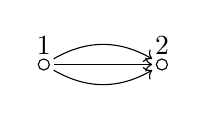
\begin{tikzpicture}[baseline = -3pt, node distance = 1.5cm]
        \node (1)                {};
        \node (2) [right of = 1] {};
        
        \draw (1) circle (2pt) node[above] {1};
        \draw (2) circle (2pt) node[above] {2};
        
        \draw[->]                  (1) edge (2);
        \draw[->, bend left  = 30] (1) edge (2);
        \draw[->, bend right = 30] (1) edge (2);
        
    \end{tikzpicture}
    $\tuple{d} = (2, 3)$, $\theta = (9, -6)$. \pause
\end{center}  
\scriptsize{
\begin{lstlisting}
julia> r, n = index(M), dimension(M)
(3, 6)

julia> H = all_weights_irreducible_component_canonical(M);

julia> for hntype in keys(H)
           H[hntype] *= -1
       end

julia> H
Dict{Vector{AbstractVector{Int64}}, Int64}:
 [[2, 2], [0, 1]]         => -30
 [[2, 1], [0, 2]]         => -40
 [[1, 0], [1, 2], [0, 1]] => -40
 [[1, 0], [1, 3]]         => -135
 [[1, 0], [1, 1], [0, 2]] => -105
 [[1, 1], [1, 2]]         => -5
 [[2, 0], [0, 3]]         => -90
\end{lstlisting}
}
\end{frame}

\begin{frame}[fragile]
    \frametitle{SOD in QuiverTools - Teleman inequality}
% \phantom{a}
\scriptsize{
\begin{lstlisting}
julia> chi = [-1, 1]; Ui = all_weights_universal_bundle(M, chi)
Dict{Vector{AbstractVector{Int64}}, Vector{Int64}}:
 [[2, 2], [0, 1]]         => [15, 0]
 [[2, 1], [0, 2]]         => [20, 10]
 [[1, 0], [1, 2], [0, 1]] => [25, 15, 10]
 [[1, 0], [1, 3]]         => [90, 45]
 [[1, 0], [1, 1], [0, 2]] => [60, 45, 30]
 [[1, 1], [1, 2]]         => [5, 0]
 [[2, 0], [0, 3]]         => [45, 30]

julia> UidualUj = all_weights_endomorphisms_universal_bundle(M);
\end{lstlisting}
}
\end{frame}

\begin{frame}[fragile]
    \frametitle{SOD in QuiverTools - Teleman inequality}
% \phantom{a}
\scriptsize{
\begin{lstlisting}
julia> all(maximum(UidualUj[hn]) - H[hn] < nu[hn] for hn in HN)
true

julia> all(maximum(-Ui[hn]) - H[hn] < nu[hn] for hn in HN)
true

julia> all(-H[hn] < nu[hn] for hn in HN)
true

julia> b = true

julia> for t in 0:r-2
        b=b && all(maximum(Ui[hn])-t*H[hn] < nu[hn] for hn in HN)
       end

julia> b
true
\end{lstlisting}
}
\end{frame}

\begin{frame}[fragile]
    \frametitle{SOD in QuiverTools - Hirzebruch--Riemann--Roch}
\scriptsize{
\begin{lstlisting}
julia> CH, CHvars = Chow_ring(M);

julia> x11, x12, x21, x22, x23 = CHvars;

julia> w=(Euler_form(Q,d,[1,0])-Euler_form(Q,[1,0],d))*x11+
         (Euler_form(Q,d,[0,1])-Euler_form(Q,[0,1],d))*x21;

julia> truncated_exp(x, n) = sum(x^i/factorial(i) for i in 0:n)

julia> Hbundle = truncated_exp(-1//r * w, n)

julia> Hbundle_dual = truncated_exp(1//r * w, n)
\end{lstlisting}
}

\end{frame}

\begin{frame}[fragile]
    \frametitle{SOD in QuiverTools - Hirzebruch--Riemann--Roch}
\scriptsize{
\begin{lstlisting}
julia> u1 = 2 + x21 + 1//2 *x11^2 - x12 + 1//6 *x11*x12 -
            1//2 *x23 - 1//8 *x23*x11 + 1//12 *x12^2 -
            1//80 * x23*x12 - 1//720 * x23^2;

julia> u1star = 2 - x21 + 1//2*x11^2 - x12 - 1//6*x11*x12 +
                1//2*x23 - 1//8*x23*x11 + 1//12*x12^2 +
                1//80 * x23*x12 - 1//720 * x23^2;

julia> u2 = 3 + x11 + 1//2*x11^2 - x22 - 1//2*x22*x11+
            2//3*x11*x12 + 1//8*x23*x11 + 1//12*x22*x12-
            1//4*x12^2 + 1//120*x23*x12;

julia> u2star = 3 - x11 + 1//2*x11^2 - x22 + 1//2*x22*x11-
                2//3*x11*x12 + 1//8*x23*x11 + 1//12*x22*x12-
                1//4*x12^2 - 1//120*x23*x12;

julia> bundles, dual_bundles = [u1, u2], [u1star, u2star];
\end{lstlisting}
}
\end{frame}

\begin{frame}[fragile]
    \frametitle{SOD in QuiverTools - Hirzebruch--Riemann--Roch}
\scriptsize{
\begin{lstlisting}
julia> m = 3;

julia> for s in 1:m-1
    println([integral(M, u*v*Hbundle_dual^s)
            for u in dual_bundles for v in bundles])
    println([integral(M, u*Hbundle_dual^s)
            for u in dual_bundles])
    println([integral(M, Hbundle_dual^s)])
    end
[0, 0, 0, 0]
[0, 0]
[0]
[0, 0, 0, 0]
[0, 0]
[0]

julia> println([integral(M, u) for u in bundles])
       println([integral(M, u*Hbundle_dual) for u in bundles])
[0, 0]
[0, 0]       
\end{lstlisting}
}
\end{frame}
% \begin{frame}
%     \frametitle{$D^b(Q)$ and $D^b(\modulispace)$.}
% [cite pieter]
% \end{frame}
\begin{frame}
    \frametitle{Decomposing quiver moduli - a QuiverTools showcase}
\begin{center}
    Thank you for your attention!
\end{center}
    

\end{frame}

\end{document}